% Block diagram of the Ethernet station, rendered to eth.png by "make
% diagrams" in the top-level Makefile. src/eth/README.md shows it. Edit
% this file, not the PNG, and render again when the entities change.
%
% What it shows: eth (eth.vhd) and the entities in it, the receive path on
% top, the three readers of the received frames in the middle, and the
% send path below, with the boundary between the PHY's clock domain and
% the system's through the two FIFOs. Each block is the VHDL entity of its
% name. It does not show the addresses, the counts of frames, the
% handshakes, or the lock that keeps the frames of the readers apart.

\documentclass[border=8pt]{standalone}

\usepackage[T1]{fontenc}
\usepackage{helvet}
\renewcommand{\familydefault}{\sfdefault}

\usepackage{tikz}
\usetikzlibrary{arrows.meta, positioning, fit, calc}

\begin{document}

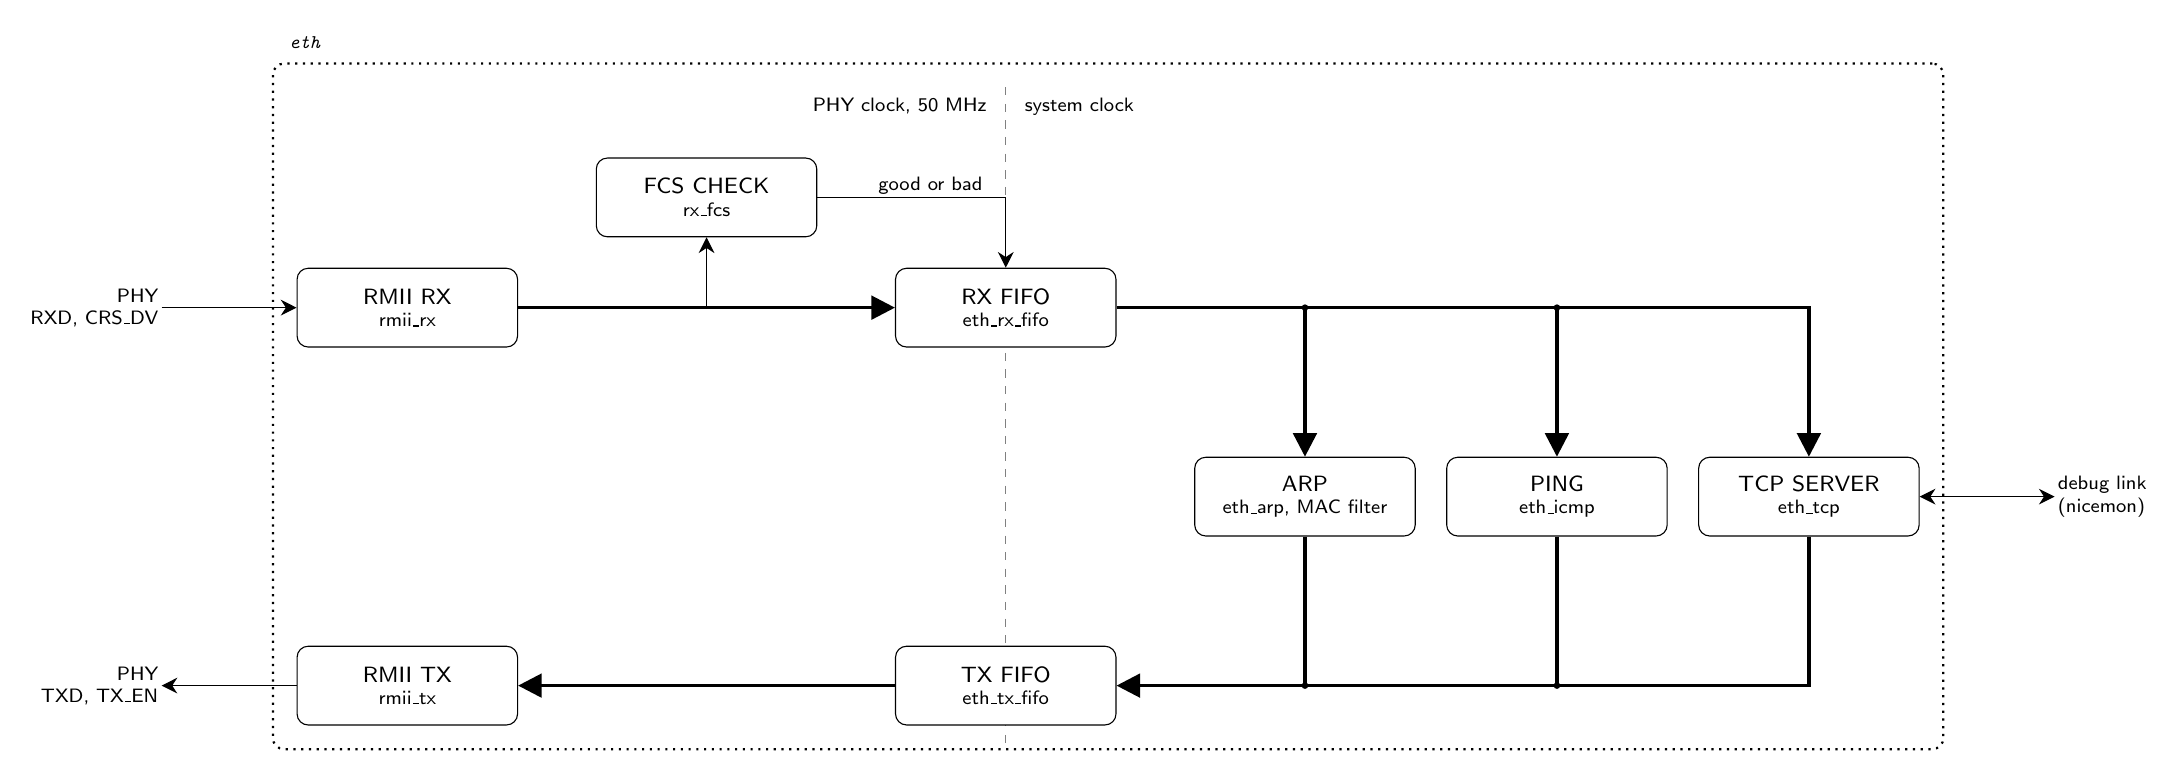
\begin{tikzpicture}[
      x = 1mm, y = 1mm,
      font = \sffamily\footnotesize,
      % A part of the station, one VHDL entity
      block/.style = {
         draw,
         rounded corners = 4pt,
         minimum width   = 28mm,
         minimum height  = 10mm,
         align           = center,
         fill            = white
      },
      % The main flow: the bytes of the frames
      flow/.style = {
         draw,
         line width = 1.2pt,
         -{Triangle[length = 3mm, width = 3mm]}
      },
      wire/.style     = {draw, -{Stealth[length = 2mm, width = 2mm]}},
      both/.style     = {draw, {Stealth[length = 2mm, width = 2mm]}-{Stealth[length = 2mm, width = 2mm]}},
      wirelabel/.style = {font = \sffamily\scriptsize, align = center, inner sep = 1pt},
      top/.style      = {draw, dotted, thick, rounded corners = 4pt, inner sep = 3mm},
      toplabel/.style = {anchor = south west, font = \ttfamily\scriptsize\itshape}
   ]

   %% ---------------------------------------------------------------
   %% The clock domains, drawn first, behind the FIFOs
   %% ---------------------------------------------------------------

   \draw[dashed, gray] (76, 28) -- (76, -56);
   \node[wirelabel, anchor = north east] at (74, 27) {PHY clock, 50 MHz};
   \node[wirelabel, anchor = north west] at (78, 27) {system clock};

   %% ---------------------------------------------------------------
   %% Receive, top
   %% ---------------------------------------------------------------

   \node[block] (rx)   at (0, 0)   {RMII RX\\[-0.5mm] {\scriptsize rmii\_rx}};
   \node[block] (fcs)  at (38, 14) {FCS CHECK\\[-0.5mm] {\scriptsize rx\_fcs}};
   \node[block] (rxf)  at (76, 0)  {RX FIFO\\[-0.5mm] {\scriptsize eth\_rx\_fifo}};

   \draw[flow] (rx) -- (rxf);
   \draw[wire] (38, 0) -- (fcs.south);
   \draw[wire] (fcs.east) -| (rxf.north)
      node[wirelabel, pos = 0.3, above] {good or bad};

   %% ---------------------------------------------------------------
   %% The three readers of the received frames, side by side
   %% ---------------------------------------------------------------

   \node[block] (arp)  at (114, -24) {ARP\\[-0.5mm] {\scriptsize eth\_arp, MAC filter}};
   \node[block] (icmp) at (146, -24) {PING\\[-0.5mm] {\scriptsize eth\_icmp}};
   \node[block] (tcp)  at (178, -24) {TCP SERVER\\[-0.5mm] {\scriptsize eth\_tcp}};

   % Every byte goes to all three
   \draw[flow] (rxf.east) -| (tcp.north);
   \draw[flow] (114, 0) -- (arp.north);
   \draw[flow] (icmp.north |- 0, 0) -- (icmp.north);
   \fill (114, 0) circle (1.2pt);
   \fill (icmp.north |- 0, 0) circle (1.2pt);

   %% ---------------------------------------------------------------
   %% Send, bottom
   %% ---------------------------------------------------------------

   \node[block] (txf)  at (76, -48) {TX FIFO\\[-0.5mm] {\scriptsize eth\_tx\_fifo}};
   \node[block] (tx)   at (0, -48)  {RMII TX\\[-0.5mm] {\scriptsize rmii\_tx}};

   \draw[flow] (tcp.south) |- (txf.east);
   \draw[flow, -] (arp.south)  -- (arp.south |- txf.east);
   \draw[flow, -] (icmp.south) -- (icmp.south |- txf.east);
   \fill (arp.south |- txf.east) circle (1.2pt);
   \fill (icmp.south |- txf.east) circle (1.2pt);
   \draw[flow] (txf) -- (tx);

   \node[top, fit = {(rx) (fcs) (tcp) (tx) (76, 28)}] (eth) {};
   \node[toplabel] at ([xshift = 1mm, yshift = 0.5mm] eth.north west) {eth};

   %% ---------------------------------------------------------------
   %% Outside: the PHY and the debug link
   %% ---------------------------------------------------------------

   \coordinate (left)  at ([xshift = -14mm] eth.west);
   \coordinate (right) at ([xshift =  14mm] eth.east);

   \draw[wire] (left |- rx.west) -- (rx.west);
   \node[wirelabel, anchor = east, align = right] at (left |- rx.west) {PHY\\ RXD, CRS\_DV};
   \draw[wire] (tx.west) -- (left |- tx.west);
   \node[wirelabel, anchor = east, align = right] at (left |- tx.west) {PHY\\ TXD, TX\_EN};

   \draw[both] (tcp.east) -- (right |- tcp.east);
   \node[wirelabel, anchor = west, align = left] at (right |- tcp.east)
      {debug link\\ (nicemon)};

\end{tikzpicture}

\end{document}
